\chapter{Ewolucyjne podejście do nieliniowego zadania transportowego}
\thispagestyle{chapterBeginStyle}

Tak jak powiedzieliśmy w poprzednim rozdziale, nieliniowe zadanie transportowe należy do zadań optymalizacyjnych, dla których trudno jest 
wyznaczyć dokładne rozwiązanie. Możemy za to za pomocą algorytmów przeszukujących zbiór dopuszczalnych rozwiązań, czyli algorytmów metaheurystycznych, 
postarać się wyznaczyć wystarczająco dobre rozwiązanie przybliżone. 

\section{Algorytmy metaheurystyczne}

Powiedzmy najpierw czym są algorytmy metaheurystyczne. Metaheurystyki są to algorytmy, które definiują sposób w jaki ma być przeszukiwany zbiór 
dopuszczalnych rozwiązań zdefiniowanego problemu. Znajdują one zastosowanie w przypadkach kiedy nie znamy algorytmów, które wyznaczają rozwiązanie 
dokładne lub ich koszt jest zbyt duży. Do tego typu problemów możemy zaliczyć rozważane tutaj nieliniowe zadanie transportowe. Minusem 
stosowania algorytmów metaheurystycznych jest fakt, że nie dają one gwarancji na znalezienie wystarczająco dobrego rozwiązania.

\subsection{Algorytmy ewolucyjne}
Algorytmy ewolucyjne stanowią podzbiór algorytmów metaheurystycznych. Sposób ich działania jest inspirowany przez zjawisko ewolucji występujące 
w naturze. Działają one na podzbiorach przestrzeni wszystkich rozwiązań, które nazywamy \textbf{populacjami}. Przy użyciu specjalnie zdefiniowanych 
operatorów, na podstawie jednej populacji tworzona jest kolejna zawierająca w sobie lepsze rozwiązania, nazywane dalej \textbf{chromosomami} 
lub \textbf{osobnikami}.

Na początku działania algorytmu generowana jest w sposób losowy populacja startowa. Procedurę generowania pojedynczego osobnika lub 
całej populacji nazywać będziemy \textbf{inicjalizacją}. Następnie na przestrzeni pokoleń (iteracji algorytmu) 
populacja ewoluuje generując coraz lepsze rozwiązania. W każdej iteracji pewna część osobników zostaje wybrana do reprodukcji. Procedurę wyboru 
rodziców do reprodukcji nazywać będziemy \textbf{selekcją}. Wybrane osobniki krzyżujemy między sobą, tworząc w ten sposób nowe, 
posiadające cechy wybranych wczesniej rodziców. Następnie losowo wybrane osobniki ulegają mutacji. 
Ostatecznie z otrzymanych osobników tworzona jest nowa populacja, która będzie stanowić bazę dla kolejnej iteracji algorytmu. Algorytm kończy 
działanie w momencie kiedy zostanie spełniony warunek końcowy, którym może być np. wygenerowanie wystarczająco dobrego rozwiązania lub 
przejście określonej liczby iteracji.

Ogólny schemat działania algorytmu ewolucyjnego przedstawiono w postaci pseudokodu \ref{alg_ewo} oraz schematu blokowego \ref{alg_ewo_img}.

\begin{pseudokod}[H]
\label{alg_ewo}
    \caption{Ogólny schemat działania algorytmu ewolucyjnego}
    $P_t$: Populacja w t-tej iteracji algorytmu\;
    $O_t$: Populacja dzieci w t-tej iteracji algorytmu\;
    \BlankLine
    $t \gets 0$\;
    inicjalizacja $P_t$\;
    \BlankLine
    \While{Warunek końcowy nie został spełniony} {
        $parents \gets$ selekcja z $P_t$\;
        $O_{t+1} \gets$ zastosuj operator krzyżowania na $parents$\;
        $O_{t+1} \gets$ zastosuj operator mutacji na $O_{t+1}$\;
        $P_{t+1} \gets$ wybierz osobniki do następnej generacji z $O_{t+1}$\;
        $t \gets t+1$\;
    }
    \Return{najlepszy osobnik z $P_t$}\;
\end{pseudokod}

\begin{figure}[H]
    \centering        
    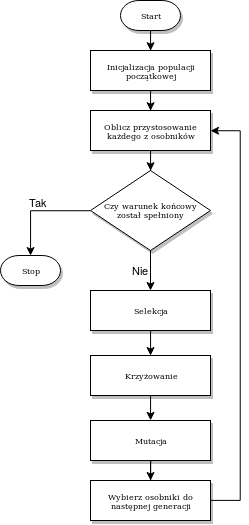
\includegraphics[width=0.6\textwidth]{img/alg_ewo_szkic.png}
    \caption{Ogólny schemat działania algorytmu ewolucyjnego.}
    \label{alg_ewo_img}
\end{figure}

Projektowanie algorytmu ewolucyjnego możemy podzielić na kilka oddzielnych części, są to: 
\begin{itemize}
    \item \textbf{Reprezentacja} - określa sposób zakodowania rozwiązania w chromosomie (osobniku). Wybór reprezentacji chromosomu jest bardzo ważnym etapem 
    projektowania algorytmu. Odpowiednia reprezentacja może w znacznym stopniu wpłynąć na szybkość i jakość rozwiązań znajdowanych przez 
    algorytm, ponieważ to ona w dużej mierze określa sposób w jaki przeszukiwana będzie przestrzeń rozwiązań zadania. 
    Jako reprezentacje bardzo często stosowane są wektory lub macierze genów, gdzie gen może być pojedynczą liczbą całkowitą lub rzeczywistą. 
    Oczywiście jako sposób reprezentacji rozwiązania możemy wybrać dowolną strukturę danych, należy jednak pamiętać, że zdefiniowane później 
    operacje mutacji i krzyżowania muszą być dostosowane do wybranej struktury.
    
    \item \textbf{Funkcja oceny} - określa stopień przystosowania danego osobnika. Bardzo często funkcja oceny jest równoważna funkcji celu, którą 
    nasz algorytm ma minimalizować/maksymalizować, nie jest to jednak regułą. 

    \item \textbf{Operator krzyżowania} - jest jednym z operatorów używanych do generowania kolejnego pokolenia w algorytmach ewolucyjnych. Z założenia 
    przyjmuje on jako argumenty dwa lub więcej rozwiązań (rodziców) i generuje na ich podstawie nowe (dzieci), które łączą w sobie cechy rodziców. 
    
    \begin{figure}[H]
        \centering        
        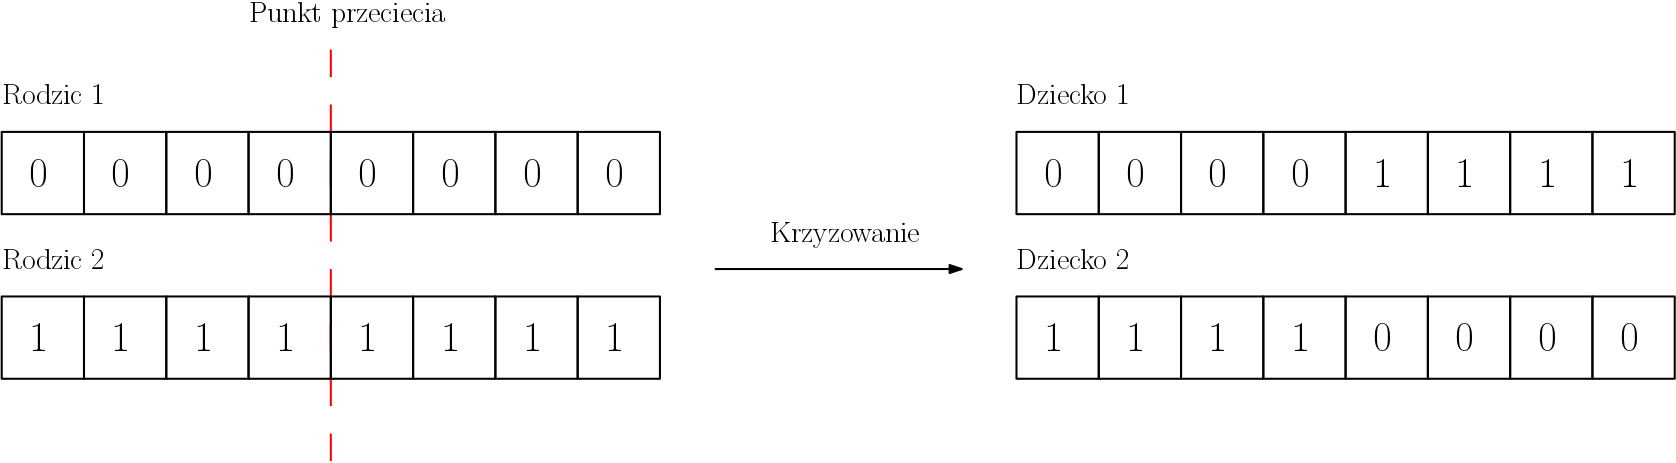
\includegraphics[width=0.9\textwidth]{img/cross_example.png}
        \caption{Przykład krzyżowania przez rozcięcie.}
    \end{figure}

    \item \textbf{Operator mutacji} - jest drugim z operatorów używanych do generowania następnych pokoleń w algorytmach ewolucyjnych. Jego celem jest 
    poszerzene obszaru przeszukiwanych rozwiązań. Ten operator powinien wprowadzać minimalną zmianę w rozwiązaniu, co zapobiega zbyt szybkiej 
    zbieżności algorytmu i pozwala na wprowadzenie dodatkowej różnorodności w populacji. Należy pamiętać o tym, że wprowadzana zmiana nie może 
    być za duża, bo może to prowadzić do odwrotnego rezultatu, czyli zamiast różnicować rozwiązania nasz operator może je niszczyć.
    
    \begin{figure}[H]
        \centering        
        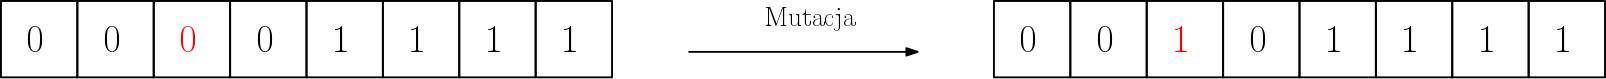
\includegraphics[width=0.9\textwidth]{img/mut_example.png}
        \caption{Przykład mutacji przez zanegowanie jednego bitu w rozwiązaniu.}
    \end{figure}

    \item \textbf{Selekcja} - określa sposób wyboru rodziców na których użyjemy operatora krzyżowania. Istnieje wiele opisanych metod selekcji\cite{SELECTION-METHODS} 
    takich jak np. metoda koła ruletki czy metoda rankingowa. Przy tworzeniu procedury selekcji należy pamiętać 
    o tym, że rozwiązania lepiej przystosowane powinny mieć większe szanse na zostanie rodzicami dla kolejnego pokolenia. Zapewnia to większe 
    szanse na wygenerowanie lepszych dzieci do następnej generacji.

    \item \textbf{Wybór następnego pokolenia} - ostateczny krok algorytmu, w którym wybieramy które osobniki wejdą w skład populacji początkowej w 
    kolejnej iteracji algorytmu. Podstawową składową tej populacji powinny być oczywiście osobniki wygenerowane za pomącą krzyżowania. Często 
    stosowaną praktyką jest również przepisywanie części najlepszych rozwiązań oraz kilku losowo wybranych z poprzedniego pokolenia. 

    \item \textbf{Parametry algorytmu} - do standardowych parametrów należą wielkość populacji, prawdopodobieństwo krzyżowania oraz prawdopodobieństwo 
    mutacji. Odpowiedni dobór parametrów ma kluczowe znaczenie dla efektywności oraz szybkości algorytmu.

\end{itemize}

W kolejnych sekcjach zaproponujemy algorytm ewolucyjny przystosowany do zadania transportowego, oparty na algorytmie zaprezentowanym przez 
dr. Zbigniewa Michalewicza\cite{ALG-GEN-BOOK}.


\section{Reprezentacja chromosomu}
W opisywanym algorytmie jako reprezentacje rozwiązania przyjęto macierz:
$$V = (v_{ij}) \text{, gdzie } 1 \le i \le length(supply) \land 1 \le j \le length(demand)$$

Rozwiązanie jest zakodowane w taki sposób, że komórka macierzy o indeksie $[i, j]$ określa ilość transportowanego towaru 
między $i$-tym punketm nadania i $j$-tym punktem odbioru. Jest to jedna z najbardziej naturalnych reprezentacji rozwiązania 
dla zadania transportowego.

\begin{table}[h!]
    \begin{center}
        \begin{tabular}{c||ccccc||c}
              & $s_1$ & $s_2$ & $s_3$ & $s_4$ & $s_5$ & $demand$ \\ 
            \hline
            \hline
            $d_1$ & 0.0 & 7.0 & 5.0 & 0.0 & 0.0 & 12.0 \\
            $d_2$ & 5.0 & 0.0 & 0.0 & 0.0 & 5.0 & 10.0 \\
            $d_3$ & 3.0 & 0.0 & 0.0 & 0.0 & 0.0 & 3.0 \\
            $d_4$ & 0.0 & 0.0 & 0.0 & 3.0 & 7.0 & 10.0 \\
            $d_5$ & 2.0 & 0.0 & 0.0 & 10.0 & 0.0 & 12.0 \\
            \hline
            \hline
            $supply$ & 10.0 & 7.0 & 5.0 & 13.0 & 12.0 & \\ 
        \end{tabular}
    \end{center}
    \caption{Przykładowe rozwiązanie.}
\end{table}

Aby ograniczenia zadania zostały zachowane, macierz rozwiązania musi spełniać następujące warunki:
$$\sum_{j=1}^{m} v_{ij} = supply[i], \text{ dla } i = 1, 2, \dots, n \text{, gdzie } n = length(supply)$$
$$\sum_{i=1}^{n} v_{ij} = demand[j], \text{ dla } j = 1, 2, \dots, m \text{, gdzie } m = length(demand)$$
$$v_{ij} \ge 0, \text{ dla } i = 1, 2, \dots, n \text{ i } j = 1, 2, \dots, m$$


\section{Inicjalizacja chromosomu}
Projektując procedurę inicjalizacji rozwiązania musimy pamiętać o tym, żeby generowane rozwiązania spełniały ograniczenia przedstawione 
w poprzedniej sekcji oraz obejmowały jak największą część przestrzeni wszystkich rozwiązań. Zaproponowana procedura przyjmuje jako argumenty 
wektory popytu i podaży. Iterując po kolejnych, losowych komórkach macierzy przypisujemy im wartość $val = \min(supply[i], demand[j])$, gdzie 
$i, j$ są indeksami wylosowanej komórki macierzy, a $supply[i]$ oraz $demand[j]$ odpowiadającymi im wartościami w wektorach popytu i podaży. 
Następnie zmniejszamy wartości w wektorach o wpisaną wartość $val$. W ten sposób ograniczenia zadania zostają spełnione. Wygenerowane rozwiązania są 
wierzchołkami sympleksu, opisującego wypukły brzeg przestrzeni dopuszczalnych rozwiązań.

\begin{pseudokod}[H]
    \label{inicjalizacja-1}
    \SetKwInOut{Input}{Wejście}
    \SetKwInOut{Output}{Wyjście}
    \caption{Procedura inicjalizacji chromosomu}
    \Input{$supply$ - wektor popytu rozmiaru $n$, $demand$ - wektor podaży rozmiaru $m$}
    \Output{$V$ - zainicjalizowana macierz}
    \BlankLine
    $V \gets zeros(n, m)$\tcc*[r]{generujemy macierz zerową rozmiaru $n \times m$}
    $indices \gets$ lista wszystkich indeksów macierzy $V$ w losowej kolejności\;
    \BlankLine
    \For{$(s, d) \in indices$} {
        $val \gets \min(demand[d], supply[s])$\;
        $demand[d] \gets demand[d] - val$\;
        $supply[s] \gets supply[s] - val$\;
        $V[s, d] \gets val$\;
    }

    \Return{$V$}
\end{pseudokod}

\begin{example}
    Przyklad inicjalizacji dla 3 dostawców i 2 odbiorców.

    1. Weźmy następujące wektory popytu i podaży:
    $$demand = [10, 12]$$
    $$supply = [8, 7, 7]$$

    2. Wygenerujmy zerową macierz rozwiązania $V$.

    $$
        V
        =
        \begin{bmatrix}
            0 & 0 & 0 \\
            0 & 0 & 0 \\
        \end{bmatrix}
    $$

    3. Wygenerujmy losowy wektor permutacji wszystkich indeksów macierzy rozwiązania.

    $$indices = [(1,1), (3,2), (1,2), (2,1), (3,1), (2,2)]$$

    4. Zainicjalizujmy komórki macierzy $V[s,d] = \min(supply[s], demand[d])$, gdzie $(s,d) \in indices$
    
    $$
        \begin{bmatrix}
            0 & 0 & 0 \\
            0 & 0 & 0 \\
        \end{bmatrix}
        \rightarrow^{(1,1)}
        \begin{bmatrix}
            \textbf{8} & 0 & 0 \\
            0 & 0 & 0 \\
        \end{bmatrix}
        \rightarrow^{(3,2)}
        \begin{bmatrix}
            8 & 0 & 0 \\
            0 & 0 & \textbf{7} \\
        \end{bmatrix}
        \rightarrow^{(1,2)}
        \begin{bmatrix}
            8 & 0 & 0 \\
            \textbf{0} & 0 & 7 \\
        \end{bmatrix}
        \rightarrow^{(2,1)}
        $$
        $$
        \begin{bmatrix}
            8 & \textbf{2} & 0 \\
            0 & 0 & 7 \\
        \end{bmatrix}
        \rightarrow^{(3,1)}
        \begin{bmatrix}
            8 & 2 & \textbf{0} \\
            0 & 0 & 7 \\
        \end{bmatrix}
        \rightarrow^{(2,2)}
        \begin{bmatrix}
            8 & 2 & 0 \\
            0 & \textbf{5} & 7 \\
        \end{bmatrix}
    $$

    5. W tym momencie kończymy procedurę inicjalizacji, nasza macierz rozwiązania ma postać:
    $$
    V
    =
    \begin{bmatrix}
        8 & 2 & 0 \\
        0 & 5 & 7 \\
    \end{bmatrix}
    $$
\end{example}


\section{Operator krzyżowania}
Operator krzyżowania został zdefiniowany jako kombinacja wypukła dwóch rodziców. W ten sposób w wyniku jednego krzyżowania powstają dwa nowe 
rozwiązania.

\begin{pseudokod}[H]
    \label{krzyżowanie}
    \SetKwInOut{Input}{Wejście}
    \SetKwInOut{Output}{Wyjście}
    \caption{Operator krzyżowania}
    \Input{$P_1, P_2$ - rodzice wybrani do krzyżowania}
    \Output{$O_1, O_2$ - otrzymane dzieci}
    \BlankLine
    $c_1 \gets rand(0,\dots,1)$\tcc*[r]{losujemy liczbę z przedziału $[0,1]$}
    $c_2 \gets 1.0 - c_1$\;
    $O_1 \gets c_1 * P_1 + c_2 * P_2$\;
    $O_2 \gets c_2 * P_1 + c_1 * P_2$\;
    \Return{$(O_1, O_2)$}\;
\end{pseudokod}

Zdefiniowany tak operator krzyżowania nie narusza ograniczeń zadania, ponieważ przestrzeń rozwiązań jest wypukła. Wynika z tego, że jeśli 
rodzice spełniali ograniczenia, to otrzymane w ten sposób dzieci również muszą spełniać ograniczenia.

\begin{example}
    Przykład zastowania operatora krzyżowania dla macierzy rozwiązania rozmiaru $3 \times 2$.

    1. Wybierzmy rodziców do krzyżowania:

    $$
        P_1
        =
        \begin{bmatrix}
            8 & 2 & 0 \\
            0 & 5 & 7 \\
        \end{bmatrix}
    $$
    $$
        P_2
        =
        \begin{bmatrix}
            0 & 3 & 7 \\
            8 & 4 & 0 \\
        \end{bmatrix}
    $$

    2. Wylosujmy współczynniki $c_1 = 0.6$ oraz $c_2 = 1 - c_1 = 0.4$

    3. Zastosujmy krzyżowanie.

    $$
        O_1
        =
        0.6
        \begin{bmatrix}
            8 & 2 & 0 \\
            0 & 5 & 7 \\
        \end{bmatrix}
        +
        0.4
        \begin{bmatrix}
            0 & 3 & 7 \\
            8 & 4 & 0 \\
        \end{bmatrix}
        =
        \begin{bmatrix}
            4.8 & 2.4 & 2.8 \\
            3.2 & 4.6 & 4.2 \\
        \end{bmatrix}
    $$
    $$
        O_2
        =
        0.4
        \begin{bmatrix}
            8 & 2 & 0 \\
            0 & 5 & 7 \\
        \end{bmatrix}
        +
        0.6
        \begin{bmatrix}
            0 & 3 & 7 \\
            8 & 4 & 0 \\
        \end{bmatrix}
        =
        \begin{bmatrix}
            3.2 & 2.6 & 4.2 \\
            4.8 & 4.4 & 2.8 \\
        \end{bmatrix}
    $$

\end{example}

\section{Operator mutacji}
Operator mutacji opiera się na modyfikacji rozwiązania poprzez wybranie z niego podmacierzy i jej ponowną inicjalizacje(patrz \ref{mutacja}). 
Załóżmy, że mamy $n$ punktów nadania i $m$ punktów odbioru. Wybierzmy jako kandydata do mutacji macierz $V = (v_{ij})$, gdzie $1 \le i \le n$ i 
$1 \le j \le m$. Podmacierz $W = w_{ij}$ jest tworzona w następujący sposób:

\begin{itemize}
    \item Losujemy podzbiór $k$ indeksów $\{i_1, \dots, i_k\}$ ze zbioru $\{1, \dots, n\}$ oraz podzbiór $l$ indeksów $\{j_1, \dots, j_l\}$ 
    ze zbioru $\{1, \dots, m\}$, $2 \le k \le n$ i $2 \le l \le m$.
    \item Tworzymy podmacierz $W$ składającą się z takich elementów macierzy $V$, które zostały wylosowane, tzn. element $v_{ij} \in V$ 
    zostaje włączony do podmacierzy $W$ tylko jeśli $i \in \{i_1, \dots, i_n\}$ oraz $j \in \{j_1, \dots, j_l\}$.
\end{itemize}

Dla stworzonej macierzy $W$ tworzymy nowe wektory $demand_W$ i $supply_W$ w następujący sposób:
$$supply_W[i] = \sum_{j \in \{j_1, \dots, j_l\}} v_{ij}, \text{ dla } 1 \le i \le k$$
$$demand_W[j] = \sum_{i \in \{i_1, \dots, i_k\}} v_{ij}, \text{ dla } 1 \le j \le l$$

Następnie na nowo inicjalizujemy podmacierz $W$ macierzy $V$ używając stworzonych wektorów $demand_W$ oraz $supply_W$ do określenia popytu i podaży 
w wybranych punktach nadania i odbioru. Po zakończeniu inicjalizacji przepisujemy wartości z podmacierzy $W$ z powrotem w odpowiadające miejsca 
macierzy $V$.

\begin{pseudokod}[H]
    \label{mutacja}
    \caption{Operator mutacji}
    \SetKwInOut{Input}{Wejście}
    \SetKwInOut{Output}{Wyjście}
    \Input{$V$ - osobnik wybrany do mutacji wielkości $n \times m$, $k, l$ - wielkość podmacierzy}
    \Output{$V$ - osobnik po mutacji}
    \BlankLine
    $supply\_idx \gets$ wylosuj podzbiór długości $k$ ze zbioru $\{1, \dots, n\}$\;
    $demand\_idx \gets$ wylosuj podzbiór długości $l$ ze zbioru $\{1, \dots, m\}$\;
    $W \gets zeros(k, l)$\tcc*[r]{generujemy macierz zerową rozmiaru $k \times l$}
    \BlankLine
    \For{$i \in \{1, \dots, k\}$} {
        \For{$j \in \{1, \dots, l\}$} {
            $W[i, j] \gets V[demand\_idx[j], supply\_idx[i]]$\;
        }
    }
    \BlankLine
    $supply\_vec \gets zeros(k)$\tcc*[r]{generujemy wektor zerowy długości k}
    $demand\_vec \gets zeros(l)$\tcc*[r]{generujemy wektor zerowy długości l}
    \BlankLine
    \For{$i \in supply\_idx$} {
        $supply\_vec[i] \gets \sum_{j \in demand\_idx} V[i, j]$\;
    }
    \BlankLine
    \For{$j \in demand\_idx$} {
        $demand\_vec[j] \gets \sum_{i \in supply\_idx} V[i, j]$\;
    }
    \BlankLine
    $W \gets inicjalizacja(W, demand\_vec, supply\_vec)$\;
    \BlankLine
    \For{$i \in \{1, \dots, k\}$} {
        \For{$j \in \{1, \dots, l\}$} {
            $V[demand\_idx[j], supply\_idx[i]] \gets W[i, j]$\;
        }
    }
    
    \Return{$V$}
\end{pseudokod}

Zdefiniowano dwa operatory mutacji. Różnią się one jedynie procedurą inicjalizacji. W pierwszym używamy tej samej procedury, którą inicjalizujemy 
nowe chromosomy podczas generowania populacji początkowej (patrz \ref{inicjalizacja-1}). Druga jest modyfikacją tej procedury. Modyfikacja polega na tym, że zamiast wybierać 
jako wartość pola $val = \min(demand[j], supply[i])$ wybieramy liczbę z zakresu $[0, val]$. Zmiana ta powoduje, że otrzymana macierz może naruszać 
ograniczenia zadania, dlatego po wstępnym wyznaczeniu wartości naprawiamy rozwiązanie poprzez zrobienie wymaganych dodawań w taki sposób, żeby 
rozwiązanie spełniało ograniczenia.

Poniżej przedstawiono schemat zmodyfikowanej procedury inicjalizacji w postaci pseudokodu.

\begin{pseudokod}[H]
    \label{inicjalizacja-2}
    \caption{Zmodyfikowana procedura inicjalizacji}
    \SetKwInOut{Input}{Wejście}
    \SetKwInOut{Output}{Wyjście}
    \Input{$supply$ - wektor podaży rozmiaru $n$, $demand$ - wektor popytu rozmiaru $m$}
    \Output{$V$ - zainicjalizowana macierz}
    \BlankLine
    $V \gets zeros(n, m)$\tcc*[r]{generujemy macierz zerową rozmiaru $n \times m$}
    $indices \gets$ lista wszystkich indeksów macierzy $V$ w losowej kolejności\;
    \BlankLine
    \For{$(s, d) \in indices$} {
        $val \gets$ wartość z przedziału $[0, \min(demand[d], supply[s])]$\;
        $demand[d] \gets demand[d] - val$\;
        $supply[s] \gets supply[s] - val$\;
        $V[s, d] \gets val$\;
    }
    \BlankLine
    \For{$(s, d) \in indices$} {
        $val \gets \min(demand[d], supply[s])$\;
        $demand[d] \gets demand[d] - val$\;
        $supply[s] \gets supply[s] - val$\;
        $V[s, d] \gets V[s, d] + val$\;
    }

    \Return{$V$}
\end{pseudokod}

\section{Funkcje oceny}
W przypadku omawianego problemu funkcja oceny jest równoważna odwrotności funkcji celu dla zadania transportowego. Powinna więc mieć postać:
$$\frac{1}{\sum_{i=1}^{n}\sum_{j=1}^{m} f(v_{ij})}$$
gdzie $f(v_{ij})$ jest dowolną funkcją przyjmującą jako argument ilość towaru transportowanego między punktami $i$ oraz $j$.
Bierzemy odwrotnośc, ponieważ chemy minimalizować funkcję celu, tzn. im mniejszy koszt osobnika, tym większa wartość funkcji przystosowania.

Przykładowe funkcje celu znajdują się w części eksperymentalnej.

\section{Metoda selekcji}
W algorytmie zastosowano standardową metodę selekcji - metodę koła ruletki. W tej metodzie lepiej przystosowane osobniki mają odpowiednio większe 
szanse na to, że zostaną wybrane do puli rodziców dla następnej generacji. Polega ona na tym, że dla każdego osobnika z populacji 
przyporzątkowujemy odpowiednio duży wycinek koła. Wielkość wycinka zależy od wartości funkcji przystosowania, jaką osiągnął dany chromosom. 
Następnie losujemy kołem tyle razy, ile rodziców chcemy otrzymać. Metoda ta pozwala na to, że jeden osobnik zostanie wybrany na rodzica kilkukrotnie.

Bardziej formalnie procedura została przedstawiona na poniższym pseudokodzie.

\begin{pseudokod}[H]
    \label{selekcja}
    \caption{Procedura selekcji}
    \SetKwInOut{Input}{Wejście}
    \SetKwInOut{Output}{Wyjście}
    \Input{$population$ - populacja chromosomów, $n$ - ilość rodziców do wybrania}
    \Output{$parents$ - wektor wybranych rodziców}
    \BlankLine
    $parents \gets$ stwórz pusty wektor długości n\;
    $k \gets length(population)$\;
    $wheel \gets zeros(k)$\tcc*[r]{Generujemy wektor zerowy długości $n$}
    \BlankLine
    $total \gets \sum_{i=1}^{k} population[i].cost$\;
    $wheel[1] \gets population[1].cost / total$\;
    \For{$i \in 2,\dots, k$} {
        $wheel[i] \gets population[i].cost / total + wheel[i-1]$\;
    }
    \BlankLine
    \For{$i \in 1,\dots, n$} {
        $num \gets rand(0,\dots, 1)$\tcc*[r]{losujemy wycinek koła}
        $selectedIdx \gets$ wybierz pierwszy taki $x$, że $wheel[x] \ge num$\;
        $parents[i] \gets population[selectedIdx]$\;
    }

    \Return{$parents$}
\end{pseudokod}

\begin{example}
    Przykład konstrukcji koła ruletki dla populacji 5 osobników. 

    Weźmy populację liczącą 5 osobników $V_1, \dots, V_5$. Niech wartość funkcji przystosowania dla osobnika $V_i$ będzie równa $c_i$.

    Załużmy, że $c_1 = 5, c_2 = 10, c_3 = 15, c_4 = 20, c_5 = 25$.

    1. Tworzymy zerowy wektor o długości równej wielkości populacji, czyli w naszym wypadku długości 5.

    $$wheel = [0, 0, 0, 0, 0]$$

    2. Sumujemy wartość funkcji przystosowania wszystkich osobników w populacji.

    $$total = \sum_{i=1}^{5} c_i = 75$$

    3. Obliczamy kolejne przedziały dla każdego z osobników.

    $$wheel[1] = c_1 / total = 0.0667$$
    $$wheel[2] = c_2 / total + wheel[1] = 0.1333 + 0.0667 = 0.2$$
    $$wheel[3] = c_3 / total + wheel[2] = 0.2 + 0.2 = 0.4$$
    $$wheel[4] = c_4 / total + wheel[3] = 0.2667 + 0.4 = 0.6667$$
    $$wheel[5] = c_5 / total + wheel[4] = 0.3333 + 0.6667 = 1$$

    4. Ostatecznie nasze koło ma postać $wheel = [0.0667, 0.2, 0.4, 0.6667, 1]$

    Teraz, aby wybrać rodzica losujemy liczbę z zakresu $[0, 1]$ i wybieramy osobnika, w którego przedziale znajduje się wylosowana liczba, np.
    załóżmy, że wylosowaliśmy liczbe $r = 0.5$. Szukamy wtedy w naszym wektorze $wheel$ takiej liczby $x \ge r$, która będzie najbliższa 
    naszemu $r$. W naszym przypadku jest to $0.6667$. Indeks wybranego rodzica jest indeksem na którym znajduje się $x$, czyli w tym wypadku $idx = 4$.
    Wybieramy więc jako rodzica osobnika $V_4$.

    Możemy łatwo zauważyć, że losując rodziców w ten sposób, osobniki z większą wartością funkcji przystosowania mają większe przedziały na kole 
    ruletki, a co za tym idzie mają wieksze szanse na to, że zostaną wybrane.
    
\end{example}

\section{Wersja równoległa}

Zaprojektowany w ten sposób algorytm możemy w dość łatwy sposób zrównoleglić. Przyjżyjmy się jeszcze raz jego strukturze. Bazą algorytmu jest 
populacja, która ewoluuje tworząc coraz lepsze, bardziej przystosowane rozwiązania. Zauważmy, że składa się ona z określonej liczby osobników, 
które są od siebie niezależne, to znaczy, że operacje wykonane na jednym osobniku populacji nie wpływają na inne osobniki. Przykładowo 
obliczając wartość funkcji przystosowania dla całej populacji nie musimy się martwić o kolejność w jakiej będziemy wybierać osobniki. Możemy więc 
podzielić populacje na mniejsze części i następnie zlecić obliczenie funkcji przystosowania poszczególnych części pojedynczym wątkom. W ten 
sposób, wszystkie części mogą być obliczane w tym samym czasie, co powinno skutkować skróceniem czasu całkowitych obliczeń dla całej populacji.

Podobnie możemy postąpić w przypadku zastosowania operatorów genetycznych, które również wpływają tylko na poszczególne osobniki, a nie na całą 
populację.

Kolejną opcją zrównoleglenia jest podział populacji na kilka mniejszych, które przez określoną liczbę pokoleń mogą ewoluować niezależnie 
od siebie. Dodatkowo dzięki temu, że częściowe populacje ewoluują niezależnie od siebie, mogą one przeszukiwać osobne części przestrzeni 
rozwiązań, co może pozytywnie wpłynąć na ostateczne rozwiązanie znalezione przez algorytm\cite{ISLAND-MODEL-PERFORMANCE}.


\subsection{Modele algorytmu}

Zaproponujmy i opiszmy dwa modele dla algorytmu:
\begin{itemize}
    \item Klasyczny
    \item Wyspowy
\end{itemize}

Na początku procedura inicjalizacji generuje losową populacje o określonej liczbie osobników i oblicza wartość funkcji oceny dla każdego z nich. 
Następnie przechodzimy do głównej pętli algorytmu, która kończy się w momencie kiedy populacja osiągnie maksymalną ilość generacji. 
Każdy z trybów różni się przebiegiem procedury \textit{nextGeneration} (patrz \ref{alg_main_img}), która tworzy nową generacje osobników.

\newpage

\begin{figure}[H]
    \centering        
    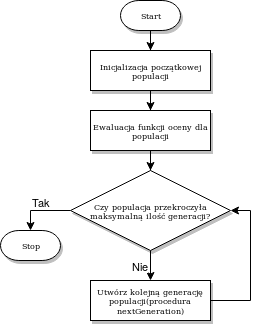
\includegraphics[width=0.6\textwidth]{img/alg_main.png}
    \caption{Przebieg zaimplementowanego algorytmu ewolucyjnego.}
    \label{alg_main_img}
\end{figure}

Model klasyczny nie różni się wiele od standardowego algorytmu ewolucyjnego. Mamy tutaj jedną populacje, która ewoluuje przez 
określoną przy starcie liczbę pokoleń. Wszystkie dostępne parametry algorytmu zostały krótko opisane w dalczej części pracy, 
w sekcji \textit{Parametry algorytmu}.

W modelu klasycznym zrównoleglenie odbywa się na poziomie pojedynczej iteracji (patrz \ref{next_gen_klasyczny_img}). 
Ewolucję populacji możemy podzielić tutaj na dwie części:
\begin{itemize}
    \item \textbf{Krzyżowanie} - w tej części między wątki rozdzielani są rodzice wybrani do krzyżowania. Następnie każdy z wątków generuje swoją część 
    dzieci oraz z określonym prawdopodobieństwem stostuje na nich operator mutacji i ostatecznie oblicza dla nich wartość funkcji oceny. 
    Dzieci są dodawane do kolejnej populacji.
    \item \textbf{Dopełnienie populacji} - w tej części do kolejnej populacji przepisywana jest część najlepszych rozwiązań oraz losowo wybranych osobników 
    z poprzedniej populacji. Następnie te dodane osobniki są poddawane mutacji i obliczana jest dla nich funkcja oceny.
\end{itemize}

\newpage

\begin{figure}[H]
    \centering        
    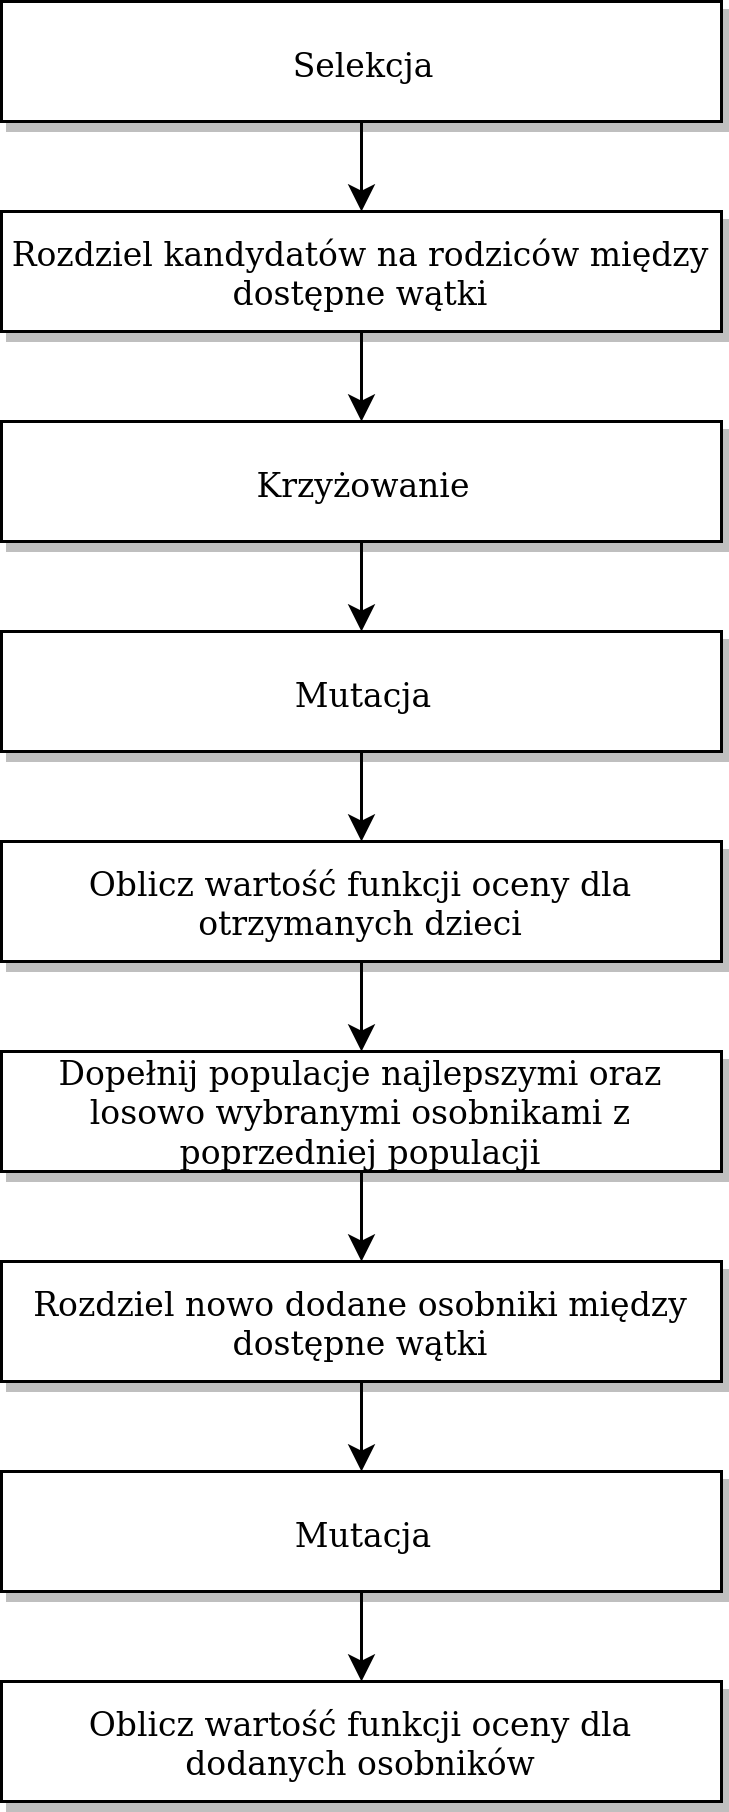
\includegraphics[width=0.4\textwidth]{img/next_gen_klasyczny.png}
    \caption{Przebieg procedury nextGeneration dla modelu klasycznego.}
    \label{next_gen_klasyczny_img}
\end{figure}

Model wyspowy różni się od klasycznego podejścia tym, że całkowita populacja jest tutaj rozdzielana na kilka mniejszych. Następnie każda z 
populacji częściowych ewoluuje niezależnie od innych przez określoną liczbę pokoleń. Po zakończeniu tego procesu wszystkie częściowe populacje 
są na nowo łączone w jedną. Następnie najlepsze rozwiązywanie jest zapisywane, a populacja zostaje na nowo podzielona na kilka mniejszych i 
cały proces się powtarza, do momentu w którym ilość generacji przekroczy określoną na początku liczbę. Na końcu najlepsze znalezione rozwiązanie 
jest zwracane.

W tym modelu zrównoleglenie obliczeń polega na tym, że przy każdym podziale populacji jeden wątek zarządza pojedynczą częścią populacji (patrz \ref{next_gen_wyspowy_img}).
Model ten skaluje się lepiej niż model klasyczny ze względu na to, że podzadania przydzielane wątkom są większe. Minusem jest tutaj to, że populacja 
musi być odpowiednio duża, żeby jej podział na mniejsze części się sprawdził.

\begin{figure}[H]
    \centering        
    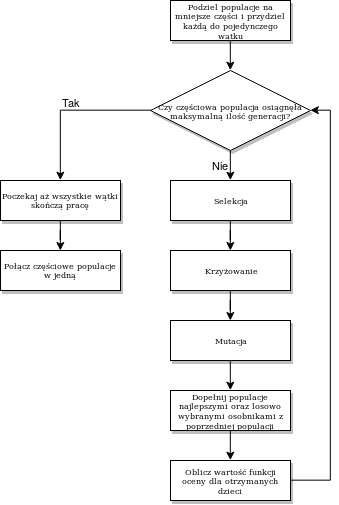
\includegraphics[width=0.7\textwidth]{img/next_gen_wyspowy.png}
    \caption{Przebieg procedury nextGeneration dla modelu wyspowego.}
    \label{next_gen_wyspowy_img}
\end{figure}

% W tym momencie każda z częściowych populacji w modelu wyspowym posiada takie same parametry. [...]

\section{Parametry algorytmu}
Opiszmy teraz krótko jakie parametry muszą zostać określone dla prezentowanego algorytmu i o czym będą one decydować.

\begin{itemize}
    \item $populationSize$ - rozmiar całkowitej populacji.
    \item $eliteProc$ - ułamek najlepszych rozwiązań, które zostają przepisane do następnego pokolenia.
    \item $mutationProb$ - prawdopodobieństwo z jaką występuje mutacja.
    \item $mutationRate$ - wielkość mutacji, określa stosunek rozmiaru podmacierzy, wybieranej do ponownej inicjalizacji podczas mutacji, 
    do macierzy rozwiązania.
    \item $crossoverProb$ - prawdopodobieństwo krzyżowania. Należy pamiętać o tym, że suma parametrów eliteProc i crossoverProb nie 
    może być większa niż $1$.
    \item $mode$ - tryb w jakim ma działać algorytm. Określa wybrany model ewolucji.
    \item $numberOfSeparateGenerations$ - określa ilość iteracji jakie wykona algorytm pomiędzy rozdzieleniem populacji na 
    mniejsze części, a ponownym jej scaleniem. Ma wpływ jedynie na model wyspowy. 
\end{itemize}

\section{Użyte technologie}
Do implementacji algorytmu zastosowano język Julia\cite{JULIA-PUB} w wersji 1.3. Julia jest stosunkowo nowym językiem programowania. Został zaprojektowany 
z myślą o zastosowaniach w obliczeniach numerycznych i analizie danych. Łączy on w sobie zalety języków niskopoziomowych i wysokopoziomowych takie jak szybkość 
i czytelność kodu. Testy pokazują, że program napisany w Julii może być równie szybki, jak odpowiadający mu program napisany w C\cite{JULIA-PERFORMANCE}. 
Dodatkową zaletą jest możliwość bezpośredniego wywoływania bibliotek napisanych w C, Fortranie i kilku innych językach popularnych w dziedzinie 
obliczeń numerycznych bezpośrednio z Julii.

Julia używa kompilatora JIT (just-in-time), który kompiluje program tuż przed jego wykonaniem, dzięki czemu jest szybsza 
niż języki interpretowane. Należy pamiętać o tym, że nie każdy program napisany w Julii będzie szybki. Wszystko zależy od jakości dostarczonego kodu.
Głównym czynnikiem, który wpływa na szybkość są typy. Julia jest językiem dynamicznie typowanym, jednak podczas kompilacji tworzone są warianty tej samej 
funkcji dla różnych typów (o ile to możliwe). Pozwala to pominąć kontrolę typów podczas wykonywania kodu i tym samym znacząco przyspieszyć jego działanie.
Dlatego pisząc kod w Julii powinniśmy pamiętać o tym, żeby unikać miejsc, w których kompilator będzie zmuszony do konwersji zmiennych do konkretnego typu. 
Aby identyfikować tego typu miejsca, możemy używać dostarczonych w bibliotece standardowej narzędzi, które pomagają analizować nasz kod. 
Warte wymienienia są tutaj:

\begin{itemize}
    \item pakiet $Profile$, który zbiera informacje o czasie wywołania kolejnych fragmentów kodu, dzięki czemu w łatwy sposób 
    możemy zidentyfikować fragmenty do dalszej optymalizacji. Pozwala on też śledzić liczbę ilość pamięci alokowanej przez konkretne fragmenty 
    kodu, co również w wielu przypadkach może okazać się przydatną informacją.
    \item makro $@code\_warntype$, które zwraca strukturę AST(abstract syntax tree) dla wykonywanego kodu, dzięki czemu możemy zobaczyć możliwe typy dla wszystkich zmiennych. 
    Dodatkowo miejsca w których kompilator nie jest w stanie jednoznacznie określić typu danej zmiennej jest zaznaczony na czerwono.
\end{itemize}

Julia udostępnia też środowisko uruchomieniowe $REPL$(read-eval-print loop), dzięki któremu możemy w bardzo łatwy sposób testować napisany kod. 
Dzięki dostępnym bibliotekom takim jak $Debugger.jl$ oraz $Rebugger.jl$ możemy w razie potrzeby debugować napisany kod z poziomu $REPL$ co 
znacznie przyspiesza znajdowanie błędów.

Ostatnie aktualizacje w znaczącym stopniu rozwinęły wsparcie języka dla obliczeń równoległych i rozproszonych. W tym momencie Julia oferuje wsparcie dla 
równoległości na poziomie wątków jak i procesów, co dodatkowo wpłynęło na wybór tego właśnie języka. Posiada własny protokół komunikacji między procesami, jednak 
istnieje również biblioteka implementująca najbardziej powszechny protokół MPI.

Biblioteka standardowa oferuje makra, które umożliwiają podział wszystkich iteracji pętli między wątki (makro $@threads$) lub procesy(makro $@distributed$). 
Taki podział zadań jest idealnym rozwiązaniem w przypadku kiedy iteracje pętli są niezależne od siebie i kolejność ich wykonywania nie ma 
znaczenia. Dokładnie taka sytuacja ma miejsce w implementowanym przez nas algorytmie, kiedy np. dzielimy populacje osobników na populacje 
częściowe, które ewoluują niezależnie od siebie. Dzięki temu mechanizm równoległości oferowany przez Julię idealnie sprawdza się w przedstawianym 
tutaj problemie.
